\chapter{Methods and techniques}%
\label{ch:methods}

\section{Choice of computational method}

As we shall see later,
good levels of theory for kinetics
require producing
\begin{enumerate*}
	\item good energies,
	\item good geometries,
	      and
	\item good vibrational frequencies.
\end{enumerate*}
Those three requirements have different demands.

One needs to choose a computational level of theory to calculate
molecular properties with accuracy.
It is important to choose a good method for the job at hand.
Many reviews are available to help one make a good decision~\cite{Goerigk_2011,Goerigk_2019,Mardirossian_2017,Morgante_2020,Bursch_2022}.
\overreact{} works with a variety of methods,
as long as the data is parseable by \texttt{cclib}~\cite{O_boyle_2008}.
It is also possible to use a combination of different levels of theory,
such as calculating geometries and frequencies with one method,
but use single-point energies with a more costly and precise one.

\citeauthor{Goerigk_2011} compared the performance of 47 density functionals
in many different applications
within the GMTKN30 dataset,
comprising 1218 single point calculations
and 841 data points of relative energies~\cite{Goerigk_2011}.
In general,
LDAs perform worse of all in all applications,
and won't be discussed further here.
Overall,
GGAs showed errors around 5.3$\pm$0.8\kcalmol,
with meta-GGAs presenting 4.4$\pm$0.6\kcalmol.
Conventional hybrid functionals performed 3.4$\pm$0.8\kcalmol,
with Minnesota hybrids following with 3.1$\pm$0.9\kcalmol,
and range-separated hybrids showing 3.3$\pm$0.5\kcalmol.
Double hybrids presented errors of 1.7$\pm$0.2\kcalmol.
All calculations were performed at essentially complete basis set
((aug-)def2-QZVP).
For comparison,
different variations of MP2
presented errors around 3.5$\pm$0.4\kcalmol.
\citeauthor{Mardirossian_2017} performed a similar
benchmark with 200 density functionals and the MGCDB84 dataset
consisting of nearly 5000 data points~\cite{Mardirossian_2017},
obtained similar results.

\citeauthor{Bursch_2022} have assembled a series of best-practices in choosing functionals for a variety of applications~\cite{Bursch_2022}.
Molecular structures can be calculated with triple-zeta basis sets (def2-TZVP)
or even well-balanced double-zeta basis sets (def2-SVP).
Geometric counterpoise (gCP,
for mitigating BSSE) and dispersion corrections are recommended in all cases (D3 or D4).
(m)GGAs are typically sufficient.
Frequencies have similar demands,
as the calculation has to be performed with an optimized geometry.

When modelling reactions,
one is often interested in reaction barrier heights.
Barrier heights refer to the amount of energy needed to move from the starting point of a reaction to the transition state,
which is the point of highest energy in the course of an elementary reaction.
As such,
one needs accurate energies for both reactants and transition state.
Transition states are challenging to calculate because they often involve weakly bound electrons
in near-degenerate molecular orbitals
due to stretched bonds,
which can lead to an underestimation of the energy barrier heights when using semi-local (m)GGA functionals.
The error is dependent on the character of bonds being broken in the transition state,
with larger errors associated with dissociation reactions,
and smaller ones with pericyclic reactions,
for instance~\cite{Bursch_2022}.
\citeauthor{Bursch_2022}~\cite{Bursch_2022} recommends the use of range-separated hybrids functionals for the calculation of reaction barriers,
as well as global hybrids (with a high amount of Fock exchange) and double hybrids,
as they mitigate self-interaction errors.
Additionally,
basis sets should be chosen carefully (oftentimes requiring triple- and quadruple-zeta basis sets) and the London dispersion energy should be taken into account~\cite{Bursch_2022}.
Finally,
for the initial search for transition states,
lower-level methods such as hybrid-based composite methods (such as PBEh-3c~\cite{Grimme_2015}) or semi-empirical methods can be used.
Further refinement can then be performed afterwards.

Finally,
in terms of electronic energies,
one can employ DLPNO-CCSD(T)~\cite{Riplinger_2013,Riplinger_2016}
in order to obtain accurate energies,
oftentimes
as good as CCSD(T).

\section{Molecular thermodynamics}

In order to perform its calculations,
\overreact{} requires the absolute Gibbs' free energies from each compound at a given temperature.
This value is calculated from
\begin{enumerate*}
	\item electronic energies,
	\item geometry coordinates,
	      and
	\item vibrational frequencies
\end{enumerate*}
of each species.
These three fundamental values are obtained
by parsing computational chemistry output files,
using the excellent \texttt{cclib} library~\cite{O_boyle_2008}.

Internally,
the library assigns a natural number for each of the $m$ chemical species,
and stores a vector $G$ of length $m$,
where each entry is an absolute Gibbs energy for that particular compound.
Absolute Gibbs energies are processed through the usual gas-phase partition-function treatment,
as explained in the subsection below.

\subsection{Partition functions}

As employed as standard in most computational chemistry packages,
the canonical gas-phase partition-function,
$q(V,
	T)$,
from statistical mechanics is employed for obtaining thermochemical properties,
which has been recommended for species in solution as well~\cite{Ribeiro_2011}.
Specifically,
the rigid-rotor harmonic oscillator (RRHO) approximation is used,
where energy levels can be decomposed into translational,
rotational,
vibrational and electronic contributions~\cite{McQuarrie_1997},
% 
\begin{equation}
	q(V,
	T) = \sum_j^\text{states} \exp \left( \frac{\epsilon_j}{k_B T} \right)
	= q_\text{trans}
	q_\text{rot}
	q_\text{vib}
	q_\text{elec}
\end{equation}
% 
where $\epsilon_j$ is an energy state,
$k_B$ is Boltzmann's constant,
$V$ is the volume,
$T$ is the temperature,
and $q_\text{trans}$,
$q_\text{rot}$,
$q_\text{vib}$ and $q_\text{elec}$ are the aforementioned total partition function contributions (with $\omega_0$ denoting spin multiplicity),
% 
\begin{equation}
	\begin{split}
		q_\text{trans}
		&= \left(
		\frac{2 \pi m k_B T}{h^2}
		\right)^\frac{3}{2}
		\frac{k_B T}{p} \\
		q_\text{rot}
		&= \begin{cases}
			% \frac{1}{\sigma}
			\frac{T}{\Theta^\text{rot}_1}
			 & \text{if linear} \\
			% \frac{1}{\sigma}
			\sqrt{
				\pi
				\frac{T^3}{
					\prod_{i = 1}^{3} \Theta^\text{rot}_i
				}
			}
			 & \text{otherwise}
		\end{cases},
		\qquad
		\Theta^\text{rot}_i = \frac{\hbar^2}{2 I_i k_B} \\
		q_\text{vib}
		&= \sum_{i = 1}^{n_\nu}
		\frac{
			\exp\left(
			- \frac{\Theta^\text{vib}_i}{2 T}
			\right)
		}{
			1 - \exp\left(
			- \frac{\Theta^\text{vib}_i
			}{T}
			\right)
		},
		\qquad
		\Theta^\text{vib}_i = \frac{h \nu_i}{k_B},
		\qquad
		n_\nu = \begin{cases}
			3 N - 5 & \text{if linear} \\
			3 N - 6 & \text{otherwise}
		\end{cases}
		\\
		q_\text{elec}
		&= \omega_0
	\end{split}
\end{equation}
% 
Observe that,
in the equations above,
molecular symmetry is not included.
They are treated separately in \overreact~(\cref{sec:mol-sym}).

From the partition functions above,
we can extract enthalpic and entropic contributions to the Gibbs free energy,
according to the well-known relations.
In practice,
vectors $U$,
$H$ and $S$,
of length $m$,
are constructed to store contributions to each species,
% 
\begin{equation}
	\begin{split}
		H_i &= U_i + p V \\
		G_i & = H_i - T S_i
	\end{split}
\end{equation}
% 
The exact contributions are given below,

\begin{subequations}
	\begin{align}
		U_\text{trans}
		 & = \frac{3}{2} R T
		 & U_\text{rot}
		 & = \begin{cases}
			     R T             & \text{if linear} \\
			     \frac{3}{2} R T & \text{otherwise}
		     \end{cases} \\
		U_\text{vib}
		 & = R \sum_{i = 1}^{n_\nu}
		\Theta^\text{vib}_i
		\left(
		\frac{1}{2}
		+ \frac{1}{
			\exp \left( \frac{\Theta^\text{vib}_i}{T}\right)
			- 1
		}
		\right)
		 & U_\text{elec}
		 & = \epsilon_{elec}
	\end{align}
	\begin{align}
		S_\text{trans}
		 & = R \left(
		\frac{5}{2}
		+ \ln{q_\text{trans}}
		\right)
		 & S_\text{elec}
		 & = R \ln{q_\text{elec}}                           \\
		S_\text{rot}
		 & = \begin{cases}
			     R \left(
			     1
			     + \ln{q_\text{rot}}
			     \right) & \text{if linear} \\
			     R \left(
			     \frac{3}{2}
			     + \ln{q_\text{rot}}
			     \right) & \text{otherwise}
		     \end{cases} \\
		S_\text{vib}
		 & = R \sum_{i = 1}^{n_\nu}
		\left[
			\frac{
				\Theta^\text{vib}_i
			}{T}
			\frac{1}{
				\exp \left( \frac{\Theta^\text{vib}_i}{T}\right)
				- 1
			}
			- \ln{\left(
				1
				- \exp \left( - \frac{\Theta^\text{vib}_i}{T}\right)
				\right)}
			\right]
	\end{align}
\end{subequations}
% 
where $\epsilon_{elec}$ stands for the final electronic energy as obtained from the output files,
which eventually includes all contributions such as dispersion and continuum solvation free energy corrections.

Further details and other treatments are detailed below.

\paragraph{Corrections to low-frequency vibrational modes}

Frequencies below 150~cm$^{-1}$ strongly contribute to entropy and must be carefully treated,
as they are known to be inaccurately treated under the RRHO approximation,
and shifts of a few wave numbers further impact the performance of the model~\cite{Ribeiro_2011,Grimme_2012,Jensen_2015,Ryu_2018}.
In order to mitigate this effect,
\overreact employs the \emph{quasi}-RRHO (QRRHO) model of~\citeauthor{Grimme_2012}~\cite{Grimme_2012},
which treats low-frequency modes as \emph{quasi}-rotations in the calculation of entropies.
In this treatment,
contributions of low-lying modes to the entropy are replaced by an interpolation between the original vibrational contributions and a corresponding rotational entropy with the moment of inertia computed for a free-rotor with reduced frequency.
The interpolation is calculated using the Head-Gordon damping function~\cite{Chai_2008},
% 
\begin{equation}
	\begin{split}
		S_\text{rot-vib,
			i}
		&= w(\nu_i) S_\text{vib,
			i}
		+ \left(
		1 - w(\nu_i)
		\right) S_\text{rot,
			i}
		\qquad
		w(\nu_i) = \frac{1}{
			1 + \left(
			\frac{
				103.6 \text{ cm}^{-1}
			}{\nu_i}
			\right)^4
		} \\
		\mu^\prime_i &= \frac{\mu_i B_\text{av}}{\mu_i + B_\text{av}},
		\qquad
		\mu_i = \frac{h}{4 \pi \nu_i},
		\qquad
		B_\text{av} = 10^{-44} \text{ kg m}^2
	\end{split}
\end{equation}
% 
A similar QRRHO treatment is also available for enthalpies~\cite{Li_2015},
where the same interpolation is employed to calculate the equivalent contribution.
Both treatments for entropies and enthalpies were tested against published results (see~\cref{fig:qrrho}).
% 
\begin{figure}[hbtp]
	\centering
	\begin{subfigure}[c]{0.5\textwidth}
		\centering
		\includegraphics[width=\textwidth]{figures/qrrho-entropy.png}
		\caption{}\label{fig:qrrho-entropy}
	\end{subfigure}%
	\begin{subfigure}[c]{0.5\textwidth}
		\centering
		\includegraphics[width=\textwidth]{figures/qrrho-enthalpy.png}
		\caption{}\label{fig:qrrho-enthalpy}
	\end{subfigure}%
	\caption{Computed (\subref{fig:qrrho-entropy})~entropy and (\subref{fig:qrrho-enthalpy})~enthalpy vibrational contributions at 298.15~K for a single mode under both RRHO and QRRHO~\cite{Grimme_2012,Li_2015} models as a function of frequency,
		as calculated by \overreact.
		The cutoff frequency for the QRRHO model was chosen as 103.6~cm$^{-1}$ and $B_\text{av} = 10^{-44}$~kg~m$^2$.
		Compare to Figures~2 and~7 of~\citeauthor{Grimme_2012}~\cite{Grimme_2012} and~\citeauthor{Li_2015}~\cite{Li_2015},
		respectively.}\label{fig:qrrho}
\end{figure}
% 
They are used by default by \overreact,
but can be deactivated by the user.

\paragraph{Low-lying imaginary frequencies}

It is not unusual to observe one or two imaginary frequencies of small magnitude in vibrational analyses,
as they are especially susceptible to numerical noise~\cite{Jensen_2015}.
This is particularly common in calculations for host-guest complexes,
weakly interacting molecules,
and other structures with flat PESs.
They can often be removed by tightening grid sizes and convergence criteria for geometry and electronic energy minimisation procedures.
In case of failure,
it is advised to consider such frequencies as real and use the corresponding thermodynamical contributions,
since excluding low-lying frequencies can result in errors as large as 2~kcal~mol$^{-1}$ at room temperature~\cite{Jensen_2015}.
As such,
\overreact highlights imaginary frequencies of small magnitude ($< 50$~cm$^{-1}$) in its output,
and makes use of their absolute value,
warning the user in the process.

\subsection{Molecular symmetries}%
\label{sec:mol-sym}

In order to calculate absolute Gibbs energies,
\overreact requires only the electronic energies,
geometries and frequencies for each species in the reaction model.

Molecular point-group symmetries are automatically detected by \overreact using a specially designed algorithm
% (manuscript in preparation)
and corrections are employed accordingly.
In practice,
a vector $\sigma$ of length $m$ is constructed consisting of the symmetry numbers~\cite{Fern_ndez_Ramos_2007,Gilson_2010} for all compounds,
and this vector is used to update all entropies,
% 
\begin{equation}
	S_i^\text{sym}
	= S_i - R \ln{\left( \sigma_i \right)}
\end{equation}
% 
% TODO: clear footnote
Extra symmetries other than the detected ones can be informed in the input by the user\footnote{See \url{https://geem-lab.github.io/overreact-guide/input.html} for a detailed input specification.},
which might be useful for,
e.g.,
weakly bound complexes~\cite{Gilson_2010} and unusual reaction path degeneracies~\cite{Fern_ndez_Ramos_2007}.

\subsection{Standard state corrections}

Quantum thermochemical calculations are usually employed in standard states,
which means 1~M for the solution phase.
On the other hand,
first-principle calculation results are reported for the gas phase,
whose standard state is 1~atm.
As such,
\overreact automatically detects (by reading the model input file) the required standard state correction to absolute Gibbs energies and applies it\footnote{See \url{https://geem-lab.github.io/overreact-guide/input.html} for a detailed input specification.},
% TODO: clear footnote
% 
\begin{equation}
	S^\text{1~M} = S^\text{1~atm}
	- R \ln{\left( \frac{c_f}{c_i} \right)}
\end{equation}
% 
where $c_f =$~1~M and $c_i$ is the concentration of an ideal gas at the given temperature and pressure.

\subsection{Adjustment of systematic errors}

First-principles microkinetic modelling is powerful and can produce meaningful and qualitatively correct results.
This is in part due to the systematic characteristic of DFT errors~\cite{P_rez_Soto_2020}.
As such,
good levels of theory often guarantee quantitative results for unimolecular reactions,
where some error cancelation is expected,
but errors can deeply affect predictions for bimolecular reactions~\cite{P_rez_Soto_2020}.
In such cases,
further adjustments can be necessary calculations of microkinetic models to be comparable to experimental results.
\overreact allows the user to adjust systematic energy errors,
which was shown to be sufficient in many cases,
when data is available~\cite{Ahn_2019,P_rez_Soto_2020}.
In particular,
\citeauthor{Schneider_2022} presents a reproduction~\cite{Schneider_2022} of the numerical results of \citeauthor{P_rez_Soto_2020}~\cite{P_rez_Soto_2020} using \overreact,
which encompasses a well-studied imine formation reaction.

\section{Automatic generation of chemical kinetic equations}

The problem of automatically generating arbitrary chemical kinetic equations is reduced to the generation of two matrices.
In \overreact,
a reaction scheme is defined as a pair of integer-valued $m \times n$-matrices $A$ and $B$,
where $n$ is the number of reactions and $m$ the number of species,
including transition states.
Entries in both matrices represent signed stoichiometric coefficients,
i.e.,
negative values denote reactants.
Both matrices $A$ and $B$ store stoichiometric coefficients for reactants,
but only $A$ stores information about products,
while only $B$ stores information about transition states.
For example,
the following system of chemical equations translate into the following matrices:
% 
\begin{equation}
	\begin{split}
		\ce{C_1 &-> C_2^{\ddagger} -> C_3} \\
		\ce{C_1 &-> C_4^{\ddagger} -> C_5} \\
	\end{split}
	\qquad
	A = \begin{bmatrix}
		-1 & -1 \\
		0  & 0  \\
		1  & 0  \\
		0  & 0  \\
		0  & 1
	\end{bmatrix}
	\qquad
	B = \begin{bmatrix}
		-1 & -1 \\
		1  & 0  \\
		0  & 0  \\
		0  & 1  \\
		0  & 0
	\end{bmatrix}
\end{equation}
% 
In this scheme,
each matrix column represents a single reaction,
while row indices indicate compounds.
For instance,
$A_{11} = A_{12} = -1$,
since \ce{C_1} is a reactant in both reactions.
The same goes for matrix $B$,
since the information regarding reactants is repeated in both matrices.
On the other hand,
$A$ stores information about products.
For instance,
$A_{31} = 1$ and $A_{52} = 1$,
since \ce{C_3} and \ce{C_5} are products of the first and second reactions,
respectively.
In the same vein,
$B$ stores information about transition states,
so $B_{21} = 1$ and $B_{42} = 1$,
since \ce{C_2$^{\ddagger}$} and \ce{C_4$^{\ddagger}$} are the respective transition states of reactions one and two.

Matrices $A$ and $B$ store all the information required for subsequent analyses.
Internally,
\overreact produce those matrices from a directed graph,
which is an idea that has proven useful in catalysis before~\cite{Kozuch_2006,Kozuch_2015,Solel_2019}.
The graph is built during input parsing in a straightforward way and both matrices $A$ and $B$ are used to generate reaction and activation Gibbs energies.

\paragraph{Equilibria}

Equilibria are treated as special forward and backward reactions obeying the equilibrium relation,
but whose reaction rate constants are always much faster than the other reactions (see~\cref{sec:rates} below).

In terms of matrix representation,
each equilibrium gives rise to \emph{two} columns in matrices $A$ and $B$.
Notwithstanding,
while the respective columns in matrix $A$ have the expected form,
matrix $B$ holds the same columns as $A$,
except for the backward reaction,
which is filled with zeroes.
This allows us to use the same machinery for calculating reaction rate constants described below,
since backward rate constants will always be unity,
while the forward constant will be numerically the same as the equilibrium constant.
A post-treatment multiplies all half-equilibria rate constants by a reasonable constant,
so that they are always faster than the other reactions in the system (see below).

As such,
\overreact does not require transition states to model equilibria,
but they are always assumed to be fast in that case.
The decision of which processes are in rapid equilibrium constitutes part of the modelling and is left to the user.
In any case,
it is advisable to provide transition states if they are known to be important,
and provide pairs of forward and backward reactions\footnote{See \url{https://geem-lab.github.io/overreact-guide/input.html} for a detailed input specification.}.
% TODO: clear footnote
On the other hand,
by providing complimentary equilibria,
complex reaction mechanisms can be properly modelled,
and many phenomena in kinetics such as pH dependencies and effects of conformations can be accounted for as simple equilibria.

\section{Reaction and activation Gibbs' free energies}

Reaction and activated Gibbs energies can be easily generated from matrices $A$ and $B$ using the $G$ vector of absolute Gibbs energies,
% 
\begin{equation}
	\begin{split}
		\Delta G &= A^T G \\
		\Delta G^\ddagger &= B^T G
	\end{split}
\end{equation}
% 
where $\Delta G$ and $\Delta G^\ddagger$ are vectors of length $n$ of reaction and activation Gibbs energies,
respectively,
and $^T$ denote matrix transposition.

\subsection{Reaction symmetries}

\overreact accounts for extra entropy contributions due to participating species being indistinguishable in a reaction.
This occurs whenever it is possible to interchangeably translate molecules of identical configurations~\cite{Fern_ndez_Ramos_2007,Gilson_2010}.
This is particularly important,
for instance,
when two identical molecules react with each other~\cite{Fern_ndez_Ramos_2007,Gilson_2010},
or when modelling explicit solvation with more than one solvent molecule (e.g.
when modelling the formation of a water cluster,
one side of the reaction would contain $n$ indistinguishable,
infinitely separated water molecules)~\cite{Jensen_2015}.
In such cases,
an extra term $-R \ln{\left( n! \right)}$ is added to the total entropy of reactants for reactions such as $\ce{n A -> products}$.

\section{Calculation of reaction rate constants}%
\label{sec:rates}

Vector $\Delta G^\ddagger$ is used to calculate a $n$-vector $k$ of reaction rate constants,
using the Eyring-Evans-Polanyi equation~\cite{Eyring_1935,Evans_1935}
% 
\begin{equation}\label{eq:rate-consts}
	k_i = \kappa_i \frac{k_B T}{h}
	\exp \left(-\frac{\Delta G_i^\ddagger}{R T} \right)
\end{equation}
% 
where $\kappa_i$ is the quantum tunnelling transmission coefficient of the $i$-th reaction (see below),
$k_B$ is Boltzmann's constant,
$h$ is Planck's constant,
$T$ is the chosen temperature and $R$ is the ideal gas constant.

Half-equilibrium reactions are assigned forward and reverse rate constants such that the equilibria is ensured,
% 
\begin{equation}
	K_\text{eq}
	% = \frac{[B]^{n_b}}{[A]^{n_a}}
	= \frac{k_i^\text{forward}}{k_{i + 1}^\text{reverse}}
	= \exp \left(-\frac{\Delta G_i}{R T} \right)
\end{equation}
% 
The slowest half-equilibrium is initially assigned unitary rate constant (see above).
Later,
after all reaction rate constants have been calculated,
all half-equilibrium reaction rates are multiplied by a factor,
such that the slowest equilibrium is at least eight times faster than the fastest non-equilibrium reaction in the model.

\subsection{Quantum tunnelling corrections}

Both Wigner~\cite{Wigner_1932} and Eckart~\cite{Eckart_1930} quantum tunnelling corrections are available for calculating $\kappa_i$ in~\cref{eq:rate-consts}.
Wigner correction is the simplest and assumes that most of the tunnelling happens at the top of the reaction barrier,
% 
\begin{equation}
	\kappa_i^\text{Wigner}
	= 1 + \frac{1}{24}
	\left(
	\frac{
		h | \nu^\ddagger |
	}{k_B T}
	\right)^2
\end{equation}
% 
where $\nu^\ddagger$,
the imaginary frequency at the transition state,
is the only information required.

The unsymmetrical Eckart correction uses information about the shape of the barrier as well,
% 
\begin{equation}
	\begin{split}
		\kappa_i^\text{Eckart}
		&= \int_{\epsilon_0}^\infty
		P(\epsilon) \exp \left(
		-\epsilon
		\right) d \epsilon,
		\qquad
		\epsilon
		= \frac{E - \Delta H^{\ddagger,
					0 K}_f}{k_B T} \\
		P(\epsilon)
		&= 1
		- \frac{
			\cosh \left(
			2 \pi (a_1 - a_2)
			\right)
			+ \cosh \left(
			2 \pi |d|
			\right)
		}{
			\cosh \left(
			2 \pi (a_1 + a_2)
			\right)
			+ \cosh \left(
			2 \pi |d|
			\right)
		} \\
		\epsilon_0 &= \begin{cases}
			-v_1 & \text{ if }
			\Delta H^{\ddagger,
					0 K}_f \le \Delta H^{\ddagger,
			0 K}_r                   \\
			-v_2 & \text{ otherwise}
		\end{cases},
		\qquad
		v_i
		= \frac{\Delta H^{\ddagger,
					0 K}_i}{k_B T} \\
		a_i
		&= \frac{
			\left[
				2
				\frac{
					\epsilon + v_i
				}{\pi u^*}
				\right]^{-\frac{1}{2}}
		}{
			\alpha_1^{-\frac{1}{2}}
			+ \alpha_2^{-\frac{1}{2}}
		},
		\qquad
		\alpha_i
		= 2 \pi \frac{
			\Delta H^{\ddagger,
					0 K}_i
		}{
			h \nu^\ddagger
		},
		\qquad
		u^*
		= \frac{
			h \nu^\ddagger
		}{
			k_B T
		} \\
		d
		&= \frac{1}{2 \pi}
		\sqrt{
			4 \alpha_1 \alpha_2 - \pi^2
		}
	\end{split}
\end{equation}
% 
where $\Delta H^{\ddagger,
			0 K}_f$ and $\Delta H^{\ddagger,
			0 K}_r$ are the activation enthalpies at 0~K for the forward and reverse reactions,
respectively.
For the integration,
we employ a carefully chosen quadrature scheme.
Eckart tunnelling corrections are employed automatically as default for all reactions,
but the user can choose Wigner or disabled it completely (in which case $\kappa_i = 1$) from the command-line\footnote{This corresponds to the \texttt{--tunneling} flag.
	See \url{https://geem-lab.github.io/overreact-guide/cli.html} for a detailed description of the command-line interface.}.

\section{Representation and solution of the kinetic ordinary differential equations}

The program generates a master equation for the entire reaction network using the reaction rate constants.
This set of ordinary differential equations (ODEs) express the rate of change of concentration of each species in the given model as a function of the instantaneous concentration of all chemical species.

The $m$-vector $y(t)$ of species concentrations (in mol/L) is time-propagated as follows.
First,
a $n$-vector of reaction rates $r(y)$,
which in general depends on $y$,
can be defined,
component-wise,
as
% 
\begin{equation}
	r_j
	= k_j \prod_i^\text{reactants}
	y_i^{-A_{ij}}
\end{equation}
% 
where the negative sign in $A_{ij}$ is due to the reactant stoichiometric coefficients being stored as negative integers.
With that definition,
$\dot{y}$ is given as
% 
\begin{equation}
	\dot{y} = A r(y)
\end{equation}
% 
where matrix multiplication is implied.

The autonomous ODE system above can be solved using any methodology.
We opted for the \texttt{SciPy} library~\cite{Virtanen_2020} for that purpose,
which provides numerically robust solvers for stiff,
non-linear systems such as the ones encountered in chemical kinetics.
Stiffness is especially true for systems with equilibrium reactions,
in which phenomena with different time scales are brought together.
The implicit Runge-Kutta method of Radau IIA family (of order five)~\cite{Hairer_1996} is used by default in \overreact,
but any solver supported by \texttt{SciPy} could be theoretically employed.
The solvers available from the command-line are \texttt{Radau},
\texttt{BDF} and \texttt{LSODA},
since these are well suited for stiff problems.

Furthermore,
a precise Jacobian for each reaction scheme is obtained by automatic differentiation provided through Google's \texttt{JAX} library~\cite{jax2018github}.
This does not only make analyses faster,
but more robust and less prone to numerical errors,
as no numerical differentiation is required throughout the microkinetic simulation.

\subsection{Concentration constraints}

Within the well-mixed condition approximation,
concentration effects are always included in microkinetic simulations.
However,
in many situations,
almost constant concentration effects are important,
such as when reactants are used neat or when there is active participation of the solvent~\cite{Ryu_2018}.
\overreact allows for fixing the concentration of an arbitrary number of compounds,
allowing for simulations of neat reactions,
pseudo-first order conditions,
pH buffering effects,
controlled ionic strengths,
and more.
Some of those applications are highlighted in \citeauthor{Schneider_2022}~\cite{Schneider_2022}.

\clearpage

% TODO: analysis of the other papers below
% TODO: merge the below

PAPER I
- Using a model substrate to elucidate reactions involving complex structures:
It is sometimes necessary to make structures smaller to make them tractable.
This has to do with the cost of the methods and there are alternatives to that as well.
- Implicit solvation models are useful,
sometimes even actual solvation molecules are important.
This has to do with the interactions that are expected to happen.
- Good models are important,
GGA/Hybrid DFTs,
etc.
There are many ways of choosing (PBE0,
etc.),
but some highlights based on benchmarks,
opinion,
etc.
- One can also correct electronic energies using even more accurate methods,
such as (DLPNO-)-CCSD(T) and others.
This requires a trick of removing the original electronic energy and using the better one.
- Counter-poise corrections can be used as well to mitigate inter- and intra-molecular basis set superposition errors.
One can do this the original way or use a semi-empirical correction such as gCP.\@

PAPER I (SI)
- Resolution of identity is useful for speeding up calculations.
- It is important to properly optimize structures
- Small imaginary frequencies can lead to some errors,
so they should be accessed and controlled.
- It is important to correct free energies to the proper
concentration when calculating for solvation phase.
This is an entropy correction and accounts to
a little over 2~\kcalmol at room temperature.
\overreact{} does this properly if the proper clue be
given in the input file.
Observe that this is an ideal correction (infinite dilution,
ideality,
etc.).
Improved treatment of entropy is a work in progress for the future,
and is \emph{hard}®.

PAPER II
- It is crucial to make use of all experimental data available (such as LC−MS and others).
- It is crucial to compare different proposed pathways.
- It is sometimes useful to compare different substrates.

PAPER II (SI)
- It is nice to start calculations with GGAs.
They might even be good enough for the whole process.
- Dispersion corrections are always needed.
- Triple-zeta basis sets are default.
- Correct energies with DLPNO-CCSD(T) whenever possible.
- gCP is cheap to use and correct BSSE.
- Use cheap methods to get initial structures,
such as xTB.
- Conformations are always useful,
Crest is good.
- NEB is a life saver if you only have reactants and products,
or you have a mild guess at the TS.
- It might be better to do NEB than OptTS sometimes.
- Scans are still useful for reactions you don't know how they end.
- In particular,
permutation problems (which water molecule?) might require
using more scans than you'd be confortable with.
- The disadvantage of a scan is that it drops in a single shot
after the barrier is found,
which might actually be useful
to \emph{find the barrier}.
- Factors revolving the preactivation complex can be
addressed by the use of dynamics.
Metadynamics is an accelerated flavor of it that
helps learning how flexible a structure is prior to reaction.
You can even infer labilities from that.
- Eckart is always better than
Wigner ($1 + \frac{1}{24} \left( \frac{h |\nu|}{R T} \right)^2$),
in my experience,
but Wigner is better than no tunneling.

PAPER III (1)
- \overreact{} takes data from computational chemistry logfiles by parsing using cclib.
- It then calculates thermodynamic properties of the compounds.
- Together with a reaction system provided by the user,
one can then calculate thermodynamic and kinetic properties of the reactions,
such as reaction rate constants.
- With the reactions and rate constants,
we build a system of ordinary differential equations
modelling the whole system.
- These equations,
along with provided initial concentrations of the species,
are used to calculate the concentrations of all species over time.

PAPER III (2)
- B97-3c is a simple model that can be used at the beginning of a study.
- Tunneling coefficients can be calculated either using Eckart or Wigner.
- UMP2 is a higher level of theory already.
- Better Pople basis sets are 6-311G(d,p) and even better 6-311G(3df,3pd),
but Pople basis sets are not recommended anymore (too much bias CITE NON-PLANAR BENZENE).
- It is my experience that,
for unimolecular reactions,
one can expect errors of around
$\pm 2 \times$ the correct reaction rate constant if using adequate levels of theory,
specially if
the quantum tunneling effects are mild.
- def2 basis set are more recommended in general than Pople.
- For stronger quantum tunneling effects,
even for unimolecular reactions,
one can have larger errors
($\pm$ one order of magnitude than the correct value,
even two in pathological cases) if the available quantum tunneling corrections are not suitable
for the given reaction,
such as if they strongly deviate from a straight line on the potential energy surface
(which is the case for ammonia umbrella inversion).
In this case,
improved barriers will help only up to a point.
If you have an unimolecular reaction
and results don't systematically improve by increasing the level of theory,
you might be experiencing this,
specially if the tunning effect is non-trivial (over two times or more).
Non-unimolecular reactions can have different diagnostics.
- Due to favourable error cancellations and the fact that
Eckart and Wigner often underestimate the quantum effects,
it is my experience that unimolecular reactions
have rate constants estimated \emph{from below},
i.e.,
the calculated values are generally lower than the
experimental ones.
Again,
Non-unimolecular reactions have different diagnostics.
- In some cases,
it is possible to obtain
values that are comparable with experimental values within 10\% of
the true reaction rate constant for gas phase reactions,
even within the experimental error values,
such as in the case
of the reproduction of Tanaka,
but one might need to have favourable error cancellations,
which might not be possible for some charge transfers,
strong electron correlations,
spin changes,
etc.
This applies to non-unimolecular reactions as well.
- Kinetic equations are stiff,
so we use proper measure to ensure they get the right treatment
- One can use equilibria together with rates when using \overreact{},
which is useful to model more complex systems.
- One can also fix the concentration of certain compounds,
which is useful
to model bulk solvent concentration (useful when it participates in the reaction),
or buffered pH conditions.
This means simulating pseudo-order reactions.
- It is oftentimes easier to correct values for equibrium constants than for reaction rates,
such as when the pK$_a$ of an acid is known
- It is oftentimes wise to use hybrid functionals when
modelling large density reorganization,
such as when charges change or
aromatic systems break or form
- One also benefits from diffuse functions when modelling charged systems
- It is wise to use dispersion corrections whenever possible.
And it is always possible.
- Non-unimolecular reactions should be treated with care
as some sources of error do not cancel gracefully,
which can lead to systematic errors.
For DFT,
these errors can be as large as 2--3~\kcalmol
when proper level of theory is employed (for the reactions investigated).
- The \emph{quasi}-rigid rotor-harmonic oscillator model
is useful to model loosely bound structures,
such as
interacting molecules,
supramolecular complexes,
etc.,
preactivation complexes,
etc.,
explicitly solvated molecules.
- Long-range separated functionals are good for weakly bound structures
or ones with weird steric effects.
- It is OK for \overreact{} to model many mechanisms at the same time.
- Tunneling effects can be important even for reactions for
which intuition would say otherwise.
- Solvent molecules should be included when it is appropriate.

PAPER III (SI)
- DONE ABOVE.\@

% TODO: check the other minor contributions after everything is done and see if we cover everything.
% Worth it.

% TODO: the rest of the text goes below.

Since the works described in~\cref{ch:paper1,ch:paper2,ch:paper3} consist
of contributions related to the computational elucidation of reaction mechanisms,
this chapter presents an account of the relevant computational methods and
techniques used in the investigations,
with background and context given
for the various topics where appropriate.
A basic background on computational chemistry applied
to mechanistic elucidation is given in~\cref{sec:background-methods}.
Details about the methods used in the development of the \overreact software
package are given in~\cref{sec:overreact-methods}.

\section{Theoretical Background}%
\label{sec:background-methods}

Each of the steps in a proposed reaction mechanism is computational modelled
by optimizing the structures of reactants,
transition states,
intermediates,
and products.
While the first two are minima on the potential energy surface,
transition
states represent a local maximum on the potential energy surface connecting
reactants and products.
This characterizes transition states as saddle points and,
therefore,
requires
a different method of optimization than the other structures.
The potential energy surface can be regarded as a function from atomic coordinates to potential energy and,
as such,
its existence is a result of the Born-Oppenheimer approximation,
where the electronic energy and wavefunction depends on the nucleus coordinates
only parametrically.
CITE BORN-OPPENHEIMER.\@
In this sense,
nuclei are treated classically in this scheme,
which is reasonable for most problems of interest in chemistry.
In contrast,
other methods exist,
where the nuclei are treated quantum mechanically as well,
but they are much more expensive.

In any case,
optimization methods require an estimate of energies and gradients
of the potential energy surface.
There are many techniques available to accomplish that,
ranging from simple and low-cost semiempirical methods,
all the way throught highly accurate and expensive multideterminantal wavefunction calculations.
CITE,
JACOB'S LADDER,
HIERARCHY OF MODELS,
ETC.\@
Most of these techniques require self-consistent field approximations,
at least initially.

The works presented in this thesis made use of the most popular technique nowadays,
the density functional theory (DFT)
method~\cite{Hohenberg_1964,Kohn_1965,Perdew_2014,Kryachko_2014,Yu_2016} for
that.
A brief discussion of the theory can be found in~\cref{sec:dft}.

\subsection{Density functional theory (DFT)}%
\label{sec:dft}

This work has made extensive use of the density functional theory (DFT).
As such,
a brief introduction to the theory is provided here.
The interested reader is invited to read the cited references for more
details~\cite{Hohenberg_1964,Kohn_1965}.

The main equation used in the DFT is the following (\cref{eq:KS}):
%
\begin{equation}
	\left(-\frac{1}{2} \laplacian
	+ v_\text{ext}
	+ v_\text{eff}
	\right) \psi_i
	= \epsilon_i \psi_i
	\label{eq:KS}
\end{equation}
%
where $\psi_i$ is $i$th molecular orbital,
$v_\text{ext}$ is the external
potential due to the atomic nuclei,
$\epsilon_i$ is the electronic energy
of the $i$th orbital and $v_\text{eff}$ is the effective potential for a given
density functional (an approximation of the actual electron-electron
interaction).
This equation is analogous to the Hartree-Fock one~\cite{Szabo_1996}
and is solved self-consistently as well.
$v_\text{eff}$ consists of classical Coulomb interactions,
as well as exchange
and correlation approximation
potentials~\cite{Perdew_2014,Kryachko_2014,Yu_2016}.
Other additive terms can appear in the potential as well,
such as solvation
approximations when employed~\cite{Marenich_2009,Marenich_2012}.
The various ways of approximating the exchange and correlation potentials give
rise to a number of density functionals developed in the
literature~\cite{Chai_2008a,Chai_2008b,Goerigk_2011,Arago_2011,Salzner_2011,Burns_2011,Minenkov_2012,DFT2016_poll}.

In the present work,
all problems were treated by expanding the molecular
orbitals as a linear combination of basis functions centered at the atomic
nuclei~\cite{Szabo_1996,Helgaker_1997,Jensen_2012,Hill_2012}.
The literature on basis set functions is extensive~\cite{Ditchfield_1971,Hehre_1972,Hariharan_1973,Hariharan_1974,Gordon_1980,Francl_1982,Clark_1983,Frisch_1984,Binning_1990,Blaudeau_1997,Rassolov_1998,Rassolov_2001}.
We invite the interested reader to the references on each work for more about
the levels of theory used in each case.

IMPACTS OF DFT APPROXIMATIONS ON THE PES?\@

\subsection{Single-molecule property predictions}%
\label{sec:optimizations}

\cref{eq:KS} allows us to obtain energy and gradient estimates (required for
the prediction of geometric,
thermochemical and kinetic properties) with a
reasonably good cost-effectiveness.
WHY,
HOW,
SUPPORT WITH WHAT?\@ CITATIONS.\@

The most basic property required for any computational study is the molecular
geometry.
It is obtained by minimizing the energy with respect to the atomic positions.
Commonly used and powerful family of optimization methods employed in the
literature is the \emph{quasi}-Newton method,
where energies and gradients are
computed,
while an approximation to the second-derivative matrix (also known as
a Hessian matrix) is updated at each step~\cite{Banerjee_1985,Schlegel_1987}.
CRUCIAL EQUATIONS SHOULD BE HIGHLIGHTED.\@

An approximation to the second-derivative matrix is employed in the algorithm
for efficiency,
but the actual matrix can be computed after the minimization is
complete.
This matrix provides important information about the region in the potential
energy surface where the energy is minimum as we will see in the following.
EVERYTHING IS MISSING,
EITHER REMOVE STUFF OR SHOW STUFF.\@
ALSO,
CITATIONS ARE LACKING.\@
DON'T APPROACH THIS TANGENTIALLY.\@

\subsubsection{Transition state optimizations}%
\label{sec:ts-optimizations}
% TODO: the logical sequence is talk about ground-state optimizations first.
% Then move to transition state optimizations.

A structure to be a minimum on the potential energy surface means that any
displacement of the structure will result in an increase in the potential
energy.
As a consequence,
its second-derivative matrix
is positive semi-definite (all eigenvalues are non-negative).
On the other hand,
first-order saddle points are characterized by behaving as
a minimum with respect to all displacements of the structure except in a single
direction.
Displacement in this particular direction leads to a decrease in the potential
energy and is associated with a single negative eigenvalue of the
second-derivative matrix.
ADD A GRAPHICAL SCHEME TO SHOW THIS.\@
By calculating the second-derivative matrix,
we can determine whether a structure
is a minimum,
saddle point or otherwise.

Obtaining transition states can be done by a number of methods.
For instance,
eigenvector following (\emph{EF})
method~\cite{Banerjee_1985,Schlegel_1987,Mauro_2005}
attempts to maximize the energy along a given promising direction,
while
minimizing the energy along all other directions.
Another much used is the \emph{STQN} method,
developed
by~Peng~and~Schlegel~\cite{Peng_1993,Peng_1996},
It consists in obtaining an estimate of the transition state from the known
structures of reactants and products (QST2).
An associated method allows the use of a custom guess for the transition state
(QST3).
% TODO: one has to list the main characteristics of each method,
% advantages and disadvantages,
% etc.
% It is nice to have equations and/or schemes to highlight the most important things and is mandatory.
The method is useful since
i.\ knowledge of the transition state is optional,
ii.\ it avoids calculating the second-derivative matrix for each step.
The nudge-elastic band method is in the same vein as the \emph{STQN} method,
but attempts to minimize a discretized trajectory connecting reactants and
products along the transition state,
and can thus make use of information about
this curve.

\subsection{Prediction of kinetics and thermodynamics for chemical reactions}

\subsubsection{Transition state theory}%
\label{sec:tst}

Transition state theory
is based on the idea that the reactant ground state complex is in equilibrium
with the transition state structure~\cite{TransitionStateTheory}.
It is summarized by the Eyring equation.

HAS TO BE REWRITTEN,
BUT ONLY THE ESSENTIALS.\@

\subsection{When things go wrong:
	bulk effects}

Here are some situations where predictions become poor due to the fact that our
calculations are too small.

FLOATING PARAGRAPH.\@

\subsubsection{Determining \emph{pKa}s}%
\label{sec:pka}

WHY?\@
THIS MAKES THE TEXT NOT FOLLOW A CONCATENATED CHAIN OF THOUGHT.\@

In the computational prediction of \emph{pKa} values,
the direct dissociation approach (\cref{eq:pKa-equilibrium})
leads to problems in the evaluation of the solvated proton,
first because it is impossible to do electronic calculations for a zero-electron
system~\cite{Ding_2009,Sumon_2012}.
%
\begin{equation}
	\ce{HB (aq) <=>[$\emph{pKa} (\ce{HB})$] B^- (aq) + H^+ (aq)}\text{.}
	\label{eq:pKa-equilibrium}
\end{equation}
%
Second,
due to the covalent nature of the interaction between the \ce{H^+} ion
and the surrounding environment,
which leads to the formation of clusters such
as \ce{H3O+},
\ce{H5O2+},
etc.~\cite{Sumon_2012}.

One can employ the experimental proton solvation free energy
($-$1104,5~$\pm$~0,3~kJ/mol~\cite{Tissandier_1998,Marenich_2009}) in a
semi-empirical fashion,
but the trustworthiness of the results is still highly
debated in the literature~\cite{Yang_2013}.
In fact,
this often produces \emph{pKa} values that are far from the expected
for simple carboxylic acids,
for instance.
Errors in the order of 7 \emph{pKa} units can be expected with this approach,
as can be found in the literature~\cite{Pliego_2002,Ding_2009}.
The major source of error can be attributed to the lack of explicit
solute-solvent interactions~\cite{Pliego_2002}.

A better approach is to use a relative determination method~\cite{Ding_2009}.
This avoids the problems associated with the direct dissociation approach
by calculating the associated problem of proton exchange with a known reference
acid,
such as acetic acid~\cite{Goldberg_2002}:
%
\begin{equation}
	\ce{HA (aq) + B^- (aq) <=>[$\Delta{} G$] HB (aq) + A^- (aq)}\text{.}
	\label{eq:pKa-indireto}
\end{equation}
%
Since both sides of the~\cref{eq:pKa-indireto}
have the same net charge and,
often both acid and conjugated base are,
in
general,
of similar structure and size,
favorable error cancelation is expected
in the Gibbs free energy ($\Delta G$).
The $\emph{pKa}(\ce{HA})$
can thus be written as a function of $\emph{pKa}(\ce{HB},
	\text{exp.})$:
%
\begin{equation}
	\emph{pKa}(\ce{HA})~=~\emph{pKa}(\ce{HB},
	\text{exp.}) + \frac{\Delta G}{\ln(10) R T}\text{.}
\end{equation}
%
It is customary that the error obtained by this method to be less than 1 \emph{pKa}
unit for many solutes and solvents~\cite{Ding_2009}.

\section{Chemical reaction mechanisms}

Hypothetical reaction mechanisms consist of
the interpretation of the available data for a chemical reaction
in terms of a model that is self-consistent.
Proposals for reaction mechanisms must be compared
with each other
and with the available experimental data.
Many different hypotheses for the same reaction can exist,
and,
after pruning the ones in disagreement with the available data,
it is still possible to have several different plausible models at hand.
Computational modelling of chemical reactions
provides one with a way of
formulating,
analyzing and
comparing hypotheses to each other,
to the literature and to the available experimental data.
This way,
one is able to come up with a ``most probable'' one.

\subsection{Bell-Evans-Polanyi principle}

The Bell-Evans-Polanyi (BEP) principle is a fundamental principle in the study
of chemical reactions.
It states that the more exothermic reactions usually have to overcome lower
reaction barriers and are therefore faster.

% TODO: equations,
% main features,
% scheme,
% missing.

It is customary to successfully extend this concept to exergonic reactions.
Notwithstanding,
since the largest contribution is the electronic energy,
it is reasonably
safe to apply the BEP principle (and Hammer's postulate,
as we will see later)
using electronic energies in the context of quantum chemistry calculations.

\subsection{Hammond's postulate}

% TODO:
THIS IS CITED IN THE INTRO AS WELL

\section{Intramolecular and substitutional effects:
  a key step to understand enzyme-like catalysis}

Despite the great advancements in the developments of artificial enzymes~\cite{Breslow_1995},
the synthetic reproduction of the reaction rate accelerations attained by
natural enzymes is far from being reached.
To get there,
we will need a more detailed comprehension of the ways enzymes
work at the molecular level~\cite{Catalysis_in_Chemistry_and_Enzymology}.
Much effort has been put in this direction,
with at least six Nobel Prizes
awarded in this and related areas~\cite{Nobel_1929,Nobel_1946,Nobel_1957,Nobel_1975,Nobel_1997,Nobel_2013}.
These progresses show that the main source of acceleration in
enzymatic reactions is to be found in the events that accompany the
enzyme-substrate complex formation that leads to bond breaking and
formation~\cite{Catalysis_in_Chemistry_and_Enzymology}.
These events induce conformational changes in both substrate and enzyme,
which
enhances the interactions in the active site~\cite{Fischer_1890,Fischer_1894,Koshland_1958,Dafforn_1971,Kirby_1996}.
PICTURES OF REPRESENTATIVE SCHEMES.\@
As a result,
substrate active centers adequately orient themselves towards
their counterparts in the active site,
which leads to
i.\ a decrease in stability of the ground state (if compared with the
free substrate state),
ii.\ a lowering of the transition state energy (if compared with the
non-catalyzed reaction),
iii.\ energy relaxation through the formation of intermediates and
products.

These driving forces are also found in intramolecular reactions (\cref{fig:reacoes-intramoleculares}).
%
\begin{figure}[hbtp]
	\centering
	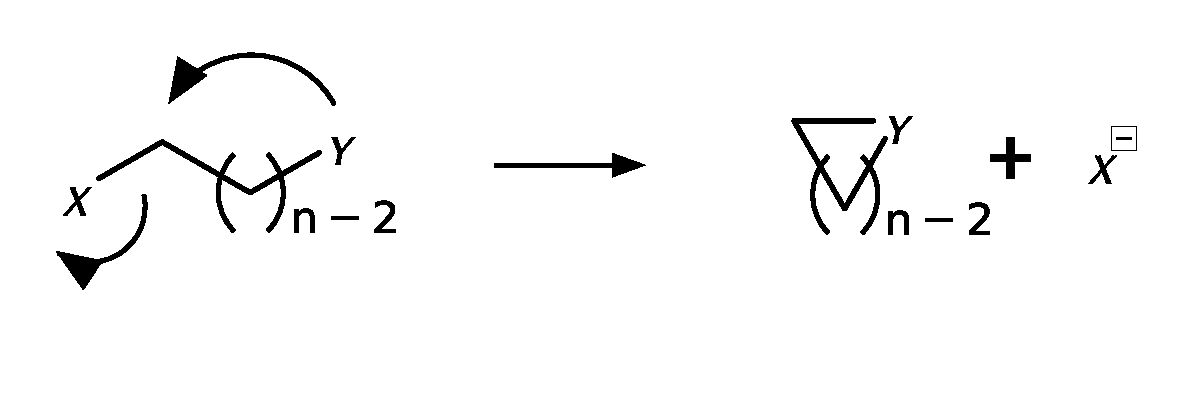
\includegraphics[width=.6\textwidth]{figures/reacao-intramolecular}
	\caption[Typical scheme of an intramolecular reactions]{
		Reaction scheme of a typical intramolecular reaction,
		whose products or
		intermediates are often cycles.
		Smaller rings ($n \le 4 $)
		tend to be disfavored by enthalpy,
		while larger rings ($n \ge 7 $)
		have less probable formation due to entropy.}%
	\label{fig:reacoes-intramoleculares}
\end{figure}
%
In fact,
the similarities between monomolecular enzymatic processes and
intramolecular reactions have been already recognized~\cite{Nilsson_1933,Bruice_1960b,Jung_1990}.
Despite the limitations of using intramolecular reactions as a model for
enzymatic reactions,
it is natural to suppose that the detailed understanding
of enzyme catalysis has,
as a prerequisite,
the ability to understand the
related processes in simpler systems.~\cite{Kirby_1972}.

We have studied some of these effects.
WHICH ONES?\@

Particular details concerning the intramolecular effects of geminal and
vicinal disubstitutions can be found in~\cref{ch:gem-vic-disubstitions}.

\section{Automatic determination of kinetics using \overreact}%
\label{sec:overreact-methods}

\overreact is an open-source library,
software package and command-line
application for building and analyzing
homogeneous microkinetic models from first-principles
calculations~\cite{Schneider_2022,overreact2021zenodo}.
It propagates chemical reactions over time using only data available from
computational chemistry calculations.

All differential equations are and their parameters are inferred from a
reaction model and calculations provided by the user.
Simultaneous reactions are easily solved,
including parallel and concurrent
reactions,
pre-equilibration and even constant concentration reactants.

Furthermore,
\overreact is able to take most of the relevant physics of the problem into
account in a semi-automated fashion.
This includes concentration effects,
symmetries,
quantum
tunneling,
standard state corrections,
implicit and explicit solvation,
proper treatment
of energy contributions and dispersion corrections.
In most cases,
in particular where solvation effects are weak,
results matching
experimental data are obtained.

% TODO: clear footnote
It is open source\footnote{Code is available at
	\url{https://github.com/geem-lab/overreact-guide}.},
free of charge,
available through the Python Package Index (PyPI) and is
distributed under the MIT license.
An online user manual is also
available\footnote{The user guide can be found at \url{https://geem-lab.github.io/overreact-guide/}.}.
% TODO: clear footnote

USE THE SI FROM THE PAPER TO ADD CONTENT HERE.\@

\section{Thermochemical partition functions}

It is possible to make use of computational calculations to obtain
thermochemical data and,
in particular,
the thermochemical partition
functions.
This is routinely achieved by standard computational chemistry packages.
This data can be used to estimate the thermodynamic properties of molecules and
whole systems.

Não apenas seus autovalores nos permitem checar se uma otimização alcançou de fato um mínimo local,
mas importantes funções de estado termodinâmicas são acessíveis através da matriz hessiana,
valendo-se da aproximação QRRHO para gases ideais.

teoria do estado de transição~\cite{TransitionStateTheory}.
%(\cref{sec:tst}).

\section{Why predicting chemical reactions is hard}

Perfect prediction of chemical reactions is an unforgiving problem.
Since reaction rate constants depend exponentially on the activation Gibbs' free energy,
small deviations on the latter exponentally increase errors on the latter.
As such,
given an activation energy estimate $\Delta G^\ddagger$
on the true value $\Delta \widehat{G}^\ddagger$
with error $\epsilon$,
%
\begin{equation}
	k = \kappa \frac{k_B T}{h} e^\frac{- \Delta G^\ddagger}{R T}
	= \kappa \frac{k_B T}{h} e^\frac{- \left(\Delta \widehat{G}^\ddagger + \epsilon\right)}{R T}
	% = \kappa \frac{k_B T}{h} e^\frac{- \Delta \widehat{G}^\ddagger}{R T}
	% e^\frac{- \epsilon}{R T}
	= \widehat{k} e^\frac{- \epsilon}{R T}
\end{equation}
%
where $k$ and $\widehat{k}$ are the predicted and true chemical reaction constants,
respectively.
Thus,
at room temperature,
an error of 1.36--2.73~\kcalmol gives rise to 10--100$\times$ error
in the reaction rate constant,
with larger errors found in lower temperatures.
This is particularly important,
as popular DFT methods commonly achieve accuracies of
2--3~\kcalmol for many molecules~\cite{Becke_2014,Bogojeski_2020}.
Moreover,
an error of 0.41~\kcalmol produces a twofold error in the constant.
This goes to show that the so called ``quantum chemical accuracy'' of
$<$1~\kcalmol~\cite{Bogojeski_2020}
is not enough for the prediction of chemical reactions on par with experimental results.
This gives rise not only to a demand
for more precise quantum chemical methods,
but also for methods aiming at mitigating the effect of such errors
in computational predictions of chemical reactions.

One might go one step further and investigate how this error in the reaction rate constant
is related to individual errors in activation enthalpy and entropy errors.
%
\begin{equation}
	k = \kappa \frac{k_B T}{h} e^\frac{- \Delta H^\ddagger}{R T}
	e^\frac{  \Delta S^\ddagger}{R}
	= \kappa \frac{k_B T}{h} e^\frac{- \left(\Delta \widehat{H}^\ddagger + \chi\right)}{R T}
	e^\frac{        \left(\Delta \widehat{S}^\ddagger + \sigma\right)}{R}
	% = \kappa \frac{k_B T}{h} e^\frac{- \Delta \widehat{H}^\ddagger}{R T}
	% e^\frac{  \Delta \widehat{S}^\ddagger}{R}
	% e^\frac{- \chi}{R T}
	% e^\frac{  \sigma}{R}
	= \widehat{k}
	e^\frac{- \chi}{R T}
	e^\frac{  \sigma}{R}
\end{equation}
%
The above suggests that,
all things equal,
errors in the predicted activation entropy dominate at high temperatures,
while being less significant
than activation enthalpy errors at low temperatures.
The balance between the two will on the other hand depend on the actual reaction at hand.

\section{``First-principle'' calculations}

Strictly speaking,
computational first-principle calculations encompass
methodologies that do not use experimental data either in their development or
application.
Broadly speaking,
the first-principle calculations can be referred to
wavefunction or density-functional theory (DFT) calculations.

Os perfis reacionais resultantes são suficientes para a predição de parâmetros
cinéticos e termodinâmicos das reações,
que foram comparados aos resultados
disponíveis na literatura.
%(\cref{sec:tst}).

\subsection{Quantum tunneling effects}

Hydrogen abstraction reactions (HAA) comprise a class of reactions where
quantum tunneling is often important~\cite{Bim2018}.
A particular group therein is the homolysis of \ce{C-H} bonds by strong
oxidants,
which oftentimes the rate-limiting step in many transformations,
and
a particularly key step in the substrate activation by numerous
metalloenzymes~\cite{Bim2018}.

\section{Microkinetic modelling}

Microkinetic modelling is a technique used to predict the outcome of complex
chemical reactions.
It can be used to investigate the catalytic transformations of molecules by
propagating a system of ordinary differential equations modelling the chemical
reactions.

The technique can be made first-principle by making use of pure computational
chemistry predictions.
It is able to take into account effects that sole use of Gibbs' free energies
are not able to,
such as concentrations of species and complex time dynamics.

\subsection{Design}

\overreact is a second iteration on an earlier attempt to build a
homogeneous microkinetic analyzer from first-principles
calculations~\cite{pyrrole2019zenodo}.
Some things were learned from that first attempt:
i.\ data is relatively easy to obtain from computational chemistry calculations,
but it is not always in its optimal form;
ii.\ solving differential equations is relatively easy in general,
but hard to
make it work for a wide range of problems mostly due to stiffness of the
equations;
iii.\ transforming knowledge about chemical structures into knowledge about the
chemical reactions is hard to be done in an automated fashion;
iv.\ having a good pipeline for data processing makes it easy to add new
features to the system.

\subsection{Automatic differentiation}

Instead of employing numerical differentiation,
whose precision depends on the
particular step size,
automatic differentiation can be used to produce
analytical derivatives in a precise,
efficient and automated way.

One conceptually simple way of doing this is by \emph{forward differentiation}
through dual numbers,
where the real values are extended by an infinitesimal
part in a trick that is not far from the concept of imaginary numbers.
The pair of numbers can be added component-wise,
and form a commutative algebra
by making use of a simple multiplication rule that follows from the property
$\epsilon^2 = 0$:
\begin{equation}
	(a,
	b) * (c,
	d)
	\equiv (a + b\epsilon)(c + d\epsilon)
	= a c + (a d + b c)\epsilon
	\equiv (a c,
	a d + b c)
\end{equation}
It is not hard to show that,
by extending the domain of any real polynomial to
dual numbers,
one obtains
\begin{equation}
	P((a,
	b)) \equiv P(a + b\epsilon) = P(a) + b P'(a) \epsilon
\end{equation}
where $P'(a)$ is the \emph{analytic} derivative of $P(a)$.

\overreact employs a sligthly more complex scheme called
\emph{backward differentiation},
available through Google's JAX library,
that
is more efficient for functions of many variables.

% TODO: highlights
Used energy correction of 3.2~kcal~mol$^{-1}$ for RMSE of 4.97~mM;\@
additional approximations (Eckart,
\emph{quasi}-rigid rotor-harmonic oscillator) applied.

% TODO: things from the quali
Mechanisms were validated on the basis of the agreement relative to respective experimental results~\cite{Kirby_1972,Jung_2005}.
The relevant thermochemistry was calculated in room temperature and atmospheric pressure (298.15~K e 1~atm).
Determinations of pK$_a$ of the studied compounds were realized with respect with acetic acid,
according to the scheme of \citeauthor{Ding_2009}~\cite{Ding_2009} (\cref{sec:pka} DO I HAVE IT?).

Calculations were realized with the program Gaussian~09C.01~\cite{g09}
and the density functional
% PBE0~\cite{Perdew_1996,Perdew_1997,Ernzerhof_1999,Adamo_1999}
\emph{wB97XD}~\cite{Chai_2008a,Chai_2008b} (\cref{sec:funcionais} DO I HAVE IT?),
which was used together with Pople basis functions with tripe-$\zeta$ quality
with diffuse and polarization functions in all atoms
(\emph{6--311++G**}~\cite{Ditchfield_1971,Hehre_1972,Hariharan_1973,Hariharan_1974,Gordon_1980,Francl_1982,Clark_1983,Frisch_1984,Binning_1990,Blaudeau_1997,Rassolov_1998,Rassolov_2001},~\cref{sec:basis-functions} DO I HAVE THIS?).
All calculations took into account aqueous solvation eefects through the use of the \emph{SMD} model,
developed by \citeauthor{Marenich_2009} (\cref{sec:implicit-solvation} DO I HAVE THIS?).
In order to investigate the effect of the geometry in the ground state,
a conformational analysis of the compounds was employed,
making use of the Open Babel 2.4.1~\cite{O_Boyle_2011}
with the \emph{PM7} model (MOPAC2016~\cite{MOPAC},~\cref{sec:conformational-analysis} DO I HAVE THIS?).

Electronic strucures of the compouds were studied under the \emph{NBO} (\cref{sec:nbos}).
In particular,
in order to orrelate the kinetic effect of the substitution
\begin{enumerate*}[label=(\roman*)]
	\item with eventual fluctuations in hybridization of the thethering carbons~\cite{Bent_1961},
	      and
	\item with the magnitude of the steric repulsion between substituents and reactive groups.
\end{enumerate*}

For that purpose,
the NBO~5.9~\cite{NBO5.9} program was utilized,
coupled with the Gaussian~09C.01~\cite{g09} software.
% TODO: things from the quali

% TODO: transform in a methodology highlight only
We showed how
acetic acid-acetate concentrations could be estimated using a combination of \emph{ab initio} calculations and experimental pK$_a$ values.
Algorithm creates fictitious reaction rate constants that guarantee equilibrium is satisfied,
allowing simultaneous study of both fast reactions and equilibria.
Equilibria can provide qualitative insight and be used to obtain Boltzmann populations with constraint optimization.
We estimated acetic acid-acetate concentrations using a combination of \emph{ab initio} calculations,
experimental pK$_a$ values and \ce{H+} concentration constraining.
Optimizations and frequencies for \ce{AcOH(aq)} system performed concluding with predictions of reaction concentrations of both solvation energies.
\overreact{} produces the expected result if given precise energy values.
% TODO: transform in a methodology highlight only

% TODO: concatenate the results with those remarks.
% It's OK not to have it all.
% PAPER 1 => is peptide-like/enzyme-like? is intramolecular/substitutional?
% PAPER 2 => is peptide-like/enzyme-like? is intramolecular/substitutional?
% PAPER 3 => is peptide-like/enzyme-like? is intramolecular/substitutional?
% => \emph{\ce{N}}-alkyl substituted maleamic acids

